\documentclass[a4paper,11pt,dvipdfmx]{ujarticle}
\usepackage{float}
% パッケージ
\usepackage{graphicx}
\usepackage{url}
% レイアウト指定を記述したファイルの読み込み
\input{layout}

% タイトルと氏名を変更せよ.
\title{日本におけるデジタル化の状況}
\author{G584212025 上田 美樹}

\begin{document}

\maketitle %ここにタイトルが入る

\section{ブロードバンドの整備状況}



OECDによるブロードバンド回線の普及に関する調査\cite{oecd}によると,図\ref{fig:imd}に示すように,
日本における100人あたりのモバイルブロードバンドの加入者数は190.5で,第1位になっている.
2位はエストニアで,3位米国と続く.

 
\begin{figure}[H]
  \centering
  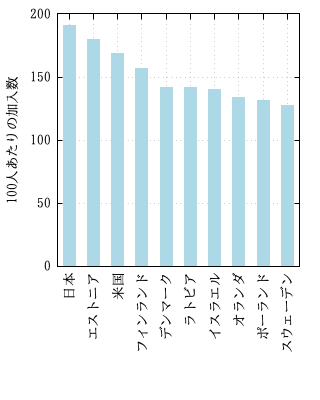
\includegraphics[width=0.6
  \linewidth]{fig21.png}
  \caption{光ファイバー回線の加入者数(100人あたり)}
  \label{fig:imd}
\end{figure}


\section{デジタル競争力ランキング}

国際経営開発研究所(IMD)の調査 \cite{imd} によると,表\ref{tab:ranking}に示すように,
日本のデジタル競争力のランキングは調査対象の64カ国中,総合で28位,知識分野で25位となっている.

\begin{table}[H]
  \centering
  \caption{デジタル競争力ランキング(64カ国中)}
  \label{tab:ranking}
  \begin{tabular}{|c|c|c|}
    \hline
    国 & 総合 & 知識 \\
    \hline
    米国 & 1位 & 3位 \\
    \hline
    香港 & 2位 & 5位 \\
    \hline
    スウェーデン & 3位 & 2位 \\
    \hline
    デンマーク & 4位 & 8位 \\
    \hline
    シンガポール & 5位 & 4位 \\
    \hline
    \hline
    韓国 & 12位 & 15位 \\
    \hline
    中国 & 15位 & 6位 \\
    \hline
    \hline
    日本 & 28位 & 25位 \\
    \hline

  \end{tabular}
\end{table}

\section{考察}
光ファイバーとデジタル競争力の関係について結果\cite{imd}から次のようなことがわかる。
\begin{itemize}
 \item 光ファイバーの加入者数が多い国は、高速で安定したインターネット環境が整っていることが多く、デジタル競争力ランキングも上位に入っている傾向がある。
 \item デジタル競争力ランキングが高い国ほど、ネットインフラが整備されているだけでなく、IT技術の活用やサービスの質も高い可能性がある。
 \item 逆に光ファイバーの加入者数が少ない国は、ネット環境の遅れからインターネット利用が制限され、生活やビジネスでのデジタル活用が遅れているケースが多い。
 \item デジタル格差の原因の一つであり、経済発展や社会のデジタル化に影響を与えていると考えられる。
\end{itemize}
今後、光ファイバーなど高速ブロードバンドのさらなる普及が進めば、デジタル競争力の向上や生活の利便性アップにつながるだろう。

\bibliographystyle{junsrt}
\bibliography{exercise.bib}

\end{document}